\section{实验六:Multithreading}\label{sec:Multithreading}

\subsection{实验目的}

\subsection{实验目的}

\begin{enumerate}
	\item 熟悉多线程编程,理解进程切换方式和执行顺序。
	\item 了解多核多线程对程序执行效率的影响。
	\item 理解锁的含义,能够判断何时、何处应该加锁。
	\item 回顾进程同步/互斥的模式并在程序中应用。 

\end{enumerate}

\subsection{实验内容}

\begin{enumerate} 
	\item 实现一个用户级进程的创建和切换。 
	\item 使用 UNIX pthread 线程库实现一个线程安全的哈希表。 
	\item 实现 barrier 函数。其作用是:当进程到达 barrier 函数调用时,会开始等待其他进程,当所有进程都到达 barrier 时,才停止等待。 
\end{enumerate}

\subsection{实验准备}

\subsubsection{多路复用}

由于操作系统需要同时运行的进程的数量可能大于电脑CPU的数量,因此需要一种让进程同时共享 CPU 的机制,理想情况下这种机制对于用户进程应该是透明的,即让每个进程都认为自己拥有一个单独的虚拟 CPU。

xv6 在 2 种情况下在进程之间切换从而实现多路复用:

\begin{enumerate}
	\item \texttt{sleep/wakeup} 机制:进程等待设备或I/O、等待子进程退出、在\texttt{sleep} sys call中等待。
	\item 周期性强迫一个进程进行切换,防止一个进程占用过长时间。 
\end{enumerate}

实现多路复用会带来一些挑战:

\begin{enumerate}
	\item 如何从一个进程切换到另一个进程?尽管上下文切换的思想很简单,但它的实现是xv6中最不透明的代码之一。
	\item 如何以对用户进程透明的方式强制切换?Xv6使用标准技术,通过定时器中断驱动上下文切换。
	\item 许多CPU可能同时在进程之间切换,使用一个用锁方案来避免争用是很有必要的。
	\item 进程退出时必须释放进程的内存以及其他资源,但它不能自己完成所有这一切,因为(例如)它不能在仍然使用自己内核栈的情况下释放它。
	\item 多核机器的每个核心必须记住它正在执行哪个进程,以便系统调用正确影响对应进程的内核状态。
	\item sleep允许一个进程放弃CPU,wakeup允许另一个进程唤醒第一个进程。需要小心避免导致唤醒通知丢失的竞争。Xv6试图尽可能简单地解决这些问题,但结果代码很复杂。  
\end{enumerate}

\begin{figure}[!htb]
	\centering
	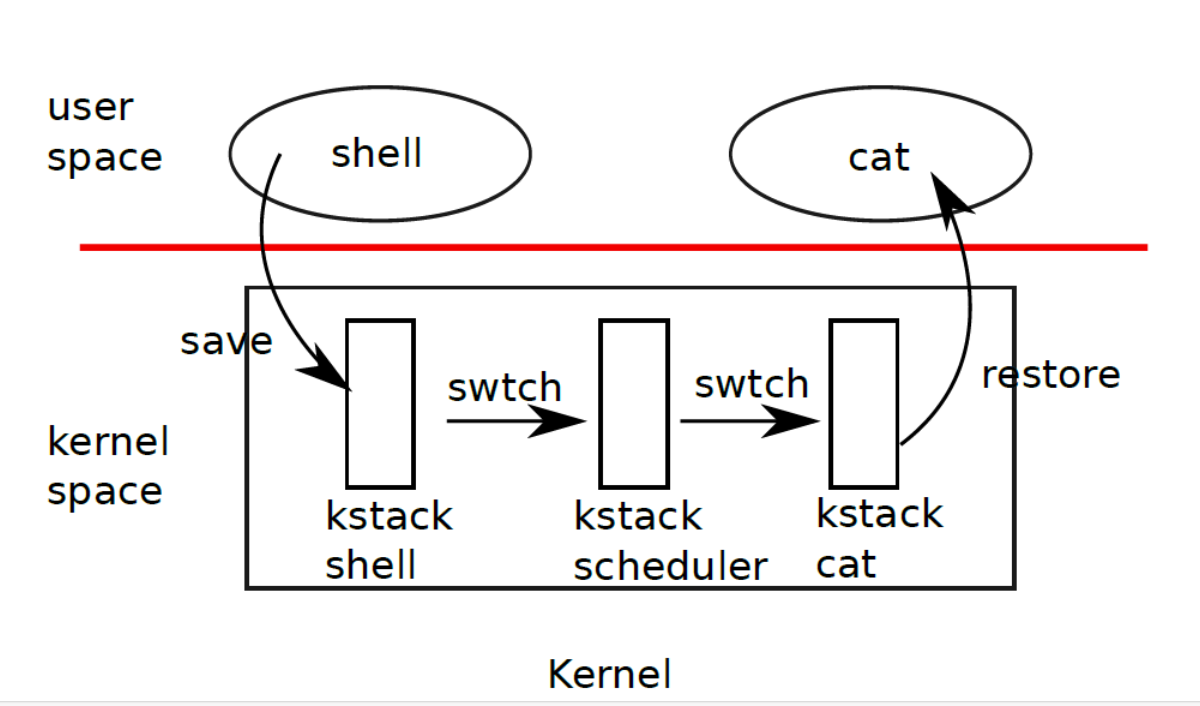
\includegraphics[width=0.6\textwidth]{multiplexing}
	\caption{从一个用户进程切换到另一个用户进程}
	\label{fig:multiplexing}
\end{figure}

\subsubsection{上下文切换}

进程的上下文切换涉及到用户空间和内核空间之间的来回转换。当进程需要切换时,首先通过系统调用或中断陷入内核态,进入该进程的内核线程,然后将内核线程的上下文切换到当前 CPU 的 scheduler 线程,再将上下文切换到需要运行的进程的内核线程,最后返回用户空间。

从一个内核线程切换到另一个线程需要保存旧线程的寄存器,恢复新线程之前保存的寄存器。\texttt{sp} 和 \texttt{pc} 将在此过程中被保存和切换。\texttt{swtch} 可以实现这种寄存器组状态的保存和切换。当进程需要 \texttt{yield} CPU 时,这个进程的内核线程将调用 \texttt{swtch} 来保存上下文并切换到 \texttt{scheduler} 的上下文,所有的上下文都保存在 \texttt{struct context} 中。\texttt{swtch} 的传入参数为 \texttt{struct context *old} 和 \texttt{struct context *new}。

yield()函数切换了进程的状态为 RUNNABLE,调用了 \texttt{sched()}。\texttt{sched} 调用了 \texttt{swtch(\&p->context, \&mycpu()->context)} 来将上下文切换到 \texttt{cpu->scheduler}。

\begin{listing}[!htb]
	\begin{minted}{c}
sched(void)
{
    int intena;
    struct proc *p = myproc();
    
    if(!holding(&p->lock))
        panic("sched p->lock");
    if(mycpu()->noff != 1)
        panic("sched locks");
    if(p->state == RUNNING)
        panic("sched running");
    if(intr_get())
        panic("sched interruptible");
    
    intena = mycpu()->intena;
    swtch(&p->context, &mycpu()->context);
    mycpu()->intena = intena;
}
	\end{minted}
	\caption{sched 函数的实现}\label{lst:sched}
\end{listing}

\texttt{sched()} 中,先要检查是否还获取着 \texttt{p->lock},防止其他 \texttt{CPU} 的 scheduler 看见 \texttt{p->state==RUNNABLE} 的情况下试图去运行这个进程。通过检查 \texttt{mycpu()->noff} 来检查是否还获取着除了 \texttt{p->lock} 之外的其他锁,否则当切换到其他进程之后其他进程可能会 \texttt{acquire} 这个锁,而原先的进程由于没有在运行,因此一直无法释放掉这个锁,造成死锁。

\texttt{swtch} 只保存 callee saved 寄存器,caller saved b寄存器在栈中被调用的代码保存。\texttt{swtch} 并没有保存 \texttt{pc} 寄存器,而是保存了 \texttt{ra},当恢复了新的进程之前保存的 \texttt{ra} 寄存器后,将返回到 \texttt{ra} 寄存器指向的上一个进程调用 \texttt{swtch} 的代码。如果保存 \texttt{pc} 寄存器,将只能回到 \texttt{swtch} 本身。由于切换到的 \texttt{\&mycpu()->context} 是被\texttt{scheduler} 对 \texttt{swtch} 的调用所保存的,因此当进行 \texttt{swtch} 时,将返回到 scheduler,栈指针也将指向当前 CPU 的 scheduler stack。

\subsubsection{调度}

调度器(scheduler)是每个CPU中都会运行的一个特殊的线程,这个线程中不断运行 \texttt{scheduler} 函数,来选取下一个需要运行的进程。

想要 \texttt{yield} 的 CPU 的进程首先要获取自己进程的锁 \texttt{p->lock}(防止其他CPU获取这个进程),修改当前的状态到 \texttt{RUNNABLE},释放掉自己获取的其他锁,加载 \texttt{cpu->scheduler} 的上下文,返回到 \texttt{scheduler()} 之后,释放掉自己的进程锁。

在 \texttt{scheduler} 调用 \texttt{swtch} 到新的进程之前,\texttt{scheduler} 需要已经获取这个进程的锁,并且将对这个进程的锁传递给被切换到的这个新的进程中,让新进程来释放这个锁。一般来说,一个锁应该由 \texttt{acquire} 它的进程来进行 \texttt{release},但是由于一个进程的 \texttt{p->state} 是在 \texttt{scheduler} 中被改变的,需要对其进行保护,因此需要在 \texttt{scheduler} 中就获取这个进程的锁。

当一个新的进程是第一次被 \texttt{scheduler} 调度的时候,不返回到 \texttt{sched},而是返回到 \texttt{forkret},因为之前并没有从sched中调用过swtch。\texttt{forkret} 将 \texttt{p->lock} 释放掉,然后回到 \texttt{usertrapret}。

\begin{listing}[!htb]
	\begin{minted}{c}
void
scheduler(void)
{
    struct proc *p;
    struct cpu *c = mycpu();

    c->proc = 0;
    for(;;){
        // Avoid deadlock by ensuring that devices can interrupt.
        intr_on();

        int nproc = 0;
        for(p = proc; p < &proc[NPROC]; p++) {
            acquire(&p->lock);
            if(p->state != UNUSED) {
                nproc++;
            }
            if(p->state == RUNNABLE) {
                // Switch to chosen process.  It is the process's job
                // to release its lock and then reacquire it
                // before jumping back to us.
                p->state = RUNNING;
                c->proc = p;
                swtch(&c->context, &p->context);
                
                // Process is done running for now.
                // It should have changed its p->state before coming back.
                c->proc = 0;
            }
            release(&p->lock);
        }
        if(nproc <= 2) {   // only init and sh exist
            intr_on();
            asm volatile("wfi");
        }
    }
}
	\end{minted}
	\caption{scheduler 函数的实现}\label{lst:scheduler}
\end{listing}

\subsubsection{mycpu 和 myproc}

xv6 每一个 CPU 都有一个 \texttt{struct cpu},记录当前运行在这个 CPU 上的进程的指针 \texttt{struct proc *proc}、保存的寄存器 \texttt{struct context context}、\texttt{push\_off} 的 nesting 的数量 \texttt{int noff} 等变量。

RISC-V 将所有 CPU 进行编号,该编号称为 hartid,确保每个 CPU 的 hartid 都保存在这个 CPU 的 \texttt{tp} 寄存器内,可以让 \texttt{mycpu} 通过这个 hartid 来索引到一个 \texttt{struct cpu} 数组 \texttt{cpus[]} 中,从而获取对当前 CPU 的 \texttt{struct cpu} 的引用。当获取 \texttt{struct cpu} 之后如果发生了中断导致 CPU 被切换了,那么获取的 \texttt{struct cpu} 将是不正确的,因此需要用 \texttt{push\_off} 来保证当前的中断使能被关闭。

使用 \texttt{myproc()} 函数来返回一个指向当前 CPU 运行的进程 \texttt{c->proc} 的指针。

\subsection{实验过程}

\subsubsection{实现用户级进程的创建和切换}

该实验要求修改 user/uthread.c 和 user/uthread\_switch.S 程序,从而实现进程间的切换。该步骤有两个要点:

\begin{enumerate}
	\item 保存被替换进程的上下文。 
	\item 恢复进入运行态进程的上下文。 
\end{enumerate}

具体实现步骤如下:

\begin{enumerate}
	\item 在 user/uthread.c 中,添加存储进程上下文的结构体 \texttt{thread\_context},并在 结构体 \texttt{thread} 中维护,如\cref{lst:add_struct_thread_context} 和  \cref{lst:add_thread_context_to_thread} 所示。
	\item 参考 kernel/Swtch.S,完成 user/uthread\_switch.S,用于保存进程上下文,如\cref{lst:uthread_switch} 所示。
	\item 在 \texttt{thread\_schedule} 中,添加对 \texttt{uthread\_switch} 的调用。如\cref{lst:use_thread_schedule_in_uthread_switch} 所示。
	\item 在 \texttt{thread\_create} 中,第一次创建进程时需要初始化 \texttt{ra} 和 \texttt{sp} 寄存器,\texttt{ra} 寄存器需要存放传入的函数地址, \texttt{sp} 寄存器传入当前线程的栈底(最开始的位置),如\cref{lst:modify_thread_create} 所示。
	\item 在 qemu 中测试 uthread,测试通过,如\cref{fig:test_uthread} 所示。
\end{enumerate}

\begin{listing}[!htb]
	\begin{minted}{c}
struct thread_context{
    uint64 ra;
    uint64 sp;
    
    uint64 s0;
    uint64 s1;
    uint64 s2;
    uint64 s3;
    uint64 s4;
    uint64 s5;
    uint64 s6;
    uint64 s7;
    uint64 s8;
    uint64 s9;
    uint64 s10;
    uint64 s11;
};
	\end{minted}
	\caption{添加 thread\_context 结构体}\label{lst:add_struct_thread_context}
\end{listing}

\begin{listing}[!htb]
	\begin{minted}{c}
struct thread {
    char       stack[STACK_SIZE]; /* the thread's stack */
    int        state;             /* FREE, RUNNING, RUNNABLE */
    struct thread_context context;
};
	\end{minted}
	\caption{在 thread 结构体中维护 thread\_context}\label{lst:add_thread_context_to_thread}
\end{listing}

\begin{listing}[!htb]
	\begin{minted}{c}
thread_switch:
/* YOUR CODE HERE */
        sd ra, 0(a0)
        sd sp, 8(a0)
        sd s0, 16(a0)
        sd s1, 24(a0)
        sd s2, 32(a0)
        sd s3, 40(a0)
        sd s4, 48(a0)
        sd s5, 56(a0)
        sd s6, 64(a0)
        sd s7, 72(a0)
        sd s8, 80(a0)
        sd s9, 88(a0)
        sd s10, 96(a0)
        sd s11, 104(a0)

        ld ra, 0(a1)
        ld sp, 8(a1)
        ld s0, 16(a1)
        ld s1, 24(a1)
        ld s2, 32(a1)
        ld s3, 40(a1)
        ld s4, 48(a1)
        ld s5, 56(a1)
        ld s6, 64(a1)
        ld s7, 72(a1)
        ld s8, 80(a1)
        ld s9, 88(a1)
        ld s10, 96(a1)
        ld s11, 104(a1)
        ret    /* return to ra */
	\end{minted}
	\caption{在 uthread\_switch 中保存上下文}\label{lst:uthread_switch}
\end{listing}

\begin{listing}[!htb]
	\begin{minted}{c}
void 
thread_schedule(void)
{
    ...
    if(current_thread != next_thread){
        next_thread->state = RUNNING;
        t = current_thread;
        current_thread = next_thread;
        thread_switch((uint64)&t->context,(uint64)&next_thread->context);
    }
    else 
        next_thread = 0;
}
	\end{minted}
	\caption{在 thread\_schedule 中调用 uthread\_switch}\label{lst:use_thread_schedule_in_uthread_switch}
\end{listing}

\begin{listing}[!htb]
	\begin{minted}{c}
void 
thread_create(void (*func)())
{
    struct thread *t;
    
    for (t = all_thread; t < all_thread + MAX_THREAD; t++) {
        if (t->state == FREE) break;
    }
    
    t->state = RUNNABLE;
    t->context.ra = (uint64)func;
    t->context.sp = (uint64) (t->stack + STACK_SIZE );
}
	\end{minted}
	\caption{完善 thread\_create 函数}\label{lst:modify_thread_create}
\end{listing}

\begin{figure}[!htb]
	\centering
	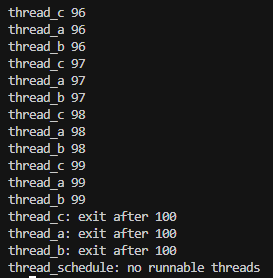
\includegraphics[width=0.5\textwidth]{test_uthread}
	\caption{测试 uthread}
	\label{fig:test_uthread}
\end{figure}

\subsubsection{实现 Using threads}

本实验与 xv6 系统代码无关,是一个使用 Unix 环境 pthread 库来学习多线程编程的练习。

\begin{enumerate}
	\item 按照说明,先运行指令 make ph,之后运行./ph 1 和./ph 2,前者正确,后者发现有丢失的键,如\cref{fig:ph1_and_ph2} 所示,说明实现有误。
	\item 声明互斥锁数组,并进行初始化,如\cref{lst:init_mutex} 所示。
	\item 在 \texttt{put} 和 \texttt{get} 函数中使用锁,如\cref{lst:use_lock_in_put_and_get}所示。
	\item 完成修改后运行./ph 2,没有丢失的键,如\cref{fig:ph1_and_ph2} 所示。
\end{enumerate}

\begin{listing}[!htb]
	\begin{minted}{c}
#define NBUCKET 5
pthread_mutex_t locks[NBUCKET];

void pthread_init_locks(){
    for(int i = 0;i<NBUCKET;i++){
        pthread_mutex_init(&locks[i],NULL);
    }
}

int
main(int argc, char *argv[])
{
    pthread_t *tha;
    void *value;
    double t1, t0;
    pthread_init_locks();
    ...
}
	\end{minted}
	\caption{声明互斥锁数组并初始化}\label{lst:init_mutex}
\end{listing}

\begin{listing}[!htb]
	\begin{minted}{c}
static 
void put(int key, int value)
{
    int i = key % NBUCKET;

    pthread_mutex_lock(&locks[i]);
    // is the key already present?
    struct entry *e = 0;
    for (e = table[i]; e != 0; e = e->next) {
        if (e->key == key)
        break;
    }

    if(e){
        // update the existing key.
        e->value = value;
    } else {
        // the new is new.
        insert(key, value, &table[i], table[i]);
    }
    pthread_mutex_unlock(&locks[i]);
}

static struct entry*
get(int key)
{
    int i = key % NBUCKET;

    pthread_mutex_lock(&locks[i]);
    
    struct entry *e = 0;
    for (e = table[i]; e != 0; e = e->next) {
        if (e->key == key) break;
    }
    pthread_mutex_unlock(&locks[i]);
    
    return e;
}
	\end{minted}
	\caption{在 put 和 get 中使用锁}\label{lst:use_lock_in_put_and_get}
\end{listing}

\begin{figure}[!htb]
	\centering
	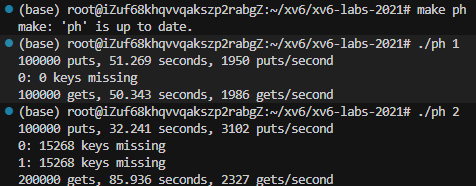
\includegraphics[width=0.6\textwidth]{ph1_and_ph2}
	\caption{修改前 ./ph 1 和 ./ph 2 的结果}
	\label{fig:ph1_and_ph2}
\end{figure}

\begin{figure}[!htb]
	\centering
	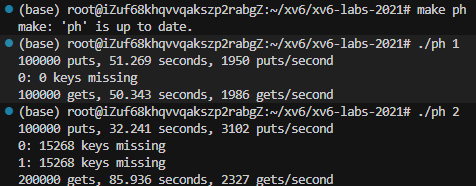
\includegraphics[width=0.6\textwidth]{ph1_and_ph2}
	
	\caption{修改后测试 ./ph 2 的结果}
	\label{fig:test_using_threads}
\end{figure}

\subsubsection{实现 Barrier}

按照说明,先运行指令 make barrier,之后运行./barrier 2,发现有错误,如\cref{fig:barrier_error} 所示,说明实现有误。

\begin{figure}[!htb]
	\centering
	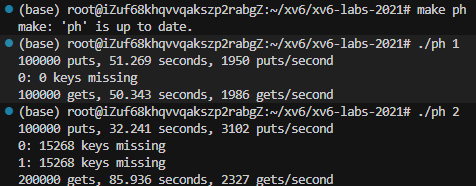
\includegraphics[width=0.6\textwidth]{ph1_and_ph2}
	\caption{修改前 ./barrier 2 的结果}
	\label{fig:barrier_error}
\end{figure}

\texttt{barrier} 函数会在所有进程都调用 \texttt{barrier} 时才解锁所有进程。通过比较 bstate.nthread 与全局变量 nthread,可以分别判断是否使进程等待或者唤醒其他进程。

\cref{lst:barrier_struct} 中各个变量的含义如下:

\begin{enumerate}
	\item \texttt{barrier\_mutex}:互斥锁,保证对 nthread 和 round 的操作是原子的,防止多线程同时修改导致数据混乱。
	\item \texttt{barrier\_cond}:条件变量,用于让线程在屏障处等待,直到所有线程都到达屏障后一起唤醒。
	\item \texttt{nthread}:记录当前有多少线程到达了屏障点。
	\item \texttt{round}:记录当前是第几轮屏障同步,方便多轮同步时判断。
\end{enumerate}

\texttt{barrier} 函数的实现过程如下,具体代码如\cref{lst:barrier} 所示:

\begin{enumerate}
	\item 加锁:所有线程进入 \texttt{barrier()} 时,先加锁,保证对共享变量的操作安全。
	\item 计数:每个线程到达屏障时,\texttt{bstate.nthread++},表示又有一个线程到达。
	\item 判断是否最后一个线程:
	 \begin{enumerate*}
	\item 如果不是最后一个到达的线程(\texttt{bstate.nthread < nthread}),就调用 \texttt{pthread\_cond\_wait} 等待,直到被唤醒。
	\item 如果是最后一个到达的线程(\texttt{bstate.nthread == nthread}),说明所有线程都到齐了:重置计数器 bstate.nthread = 0,为下一轮屏障做准备。屏障轮次加一 \texttt{bstate.round++}。用 \texttt{pthread\_cond\_broadcast} 唤醒所有在等待的线程。
	\end{enumerate*}
	\item 解锁:所有线程被唤醒后,解锁,继续执行后续代码。
\end{enumerate}

\begin{listing}[!htb]
	\begin{minted}{c}
struct barrier {
    pthread_mutex_t barrier_mutex;
    pthread_cond_t barrier_cond;
    int nthread;      // Number of threads that have reached this round of the barrier
    int round;     // Barrier round
} bstate;
	\end{minted}
	\caption{barrier 结构体}\label{lst:barrier_struct}
\end{listing}

\begin{listing}[!htb]
	\begin{minted}{c}
static void 
barrier()
{
    pthread_mutex_lock(&bstate.barrier_mutex);
    bstate.nthread++;
    
    if(bstate.nthread < nthread){
        pthread_cond_wait(&bstate.barrier_cond, &bstate.barrier_mutex);
    }
    else{
        bstate.nthread = 0;
        bstate.round++;
        pthread_cond_broadcast(&bstate.barrier_cond);
    }
    pthread_mutex_unlock(&bstate.barrier_mutex);
}
	\end{minted}
	\caption{barrier 函数的实现}\label{lst:barrier}
\end{listing}

\begin{figure}[!htb]
	\centering
	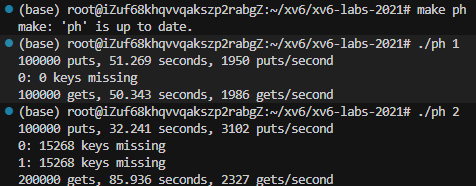
\includegraphics[width=0.5\textwidth]{ph1_and_ph2}
	\caption{测试 barrier}
	\label{fig:test_barrier}
\end{figure}

\subsubsection{综合测试}

在 xv6-labs-2021 目录下创建一个time.txt文件,记录该lab花费的时间,再创建一个answers-threads.txt 文件,记录对lab中问题的解答。使用 \texttt{make grade} 对lab6进行综合测试,测试通过。

\begin{figure}[!htb]
	\centering
	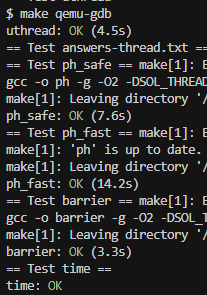
\includegraphics[width=0.4\textwidth]{test_lab6}
	\caption{测试 lab6}
	\label{fig:test_lab6}
\end{figure}

\subsection{实验小结}

本实验是关于多线程编程的。之前并没有编写过多线程的程序,只知道多线程程序可以运用多个处理器,可以达到提高速度的效果。在操作系统课程中介绍了锁的概念和几个模型,并讨论了多线程存在的死锁问题。在实验中,实现了进程切换、运用锁来完成线程间的互斥(多线程哈希表)和运用锁和条件信号量来完成多线程之间的同步(barrier),三个小实验加深了我对于多线程的理解,提供了练习多线程编程的机会。 